\chapter{Key-value model, MapReduce and Hadoop} % (fold)
\label{cha:background}

This chapter introduces some concepts that are used in the subsequent sections:
the key-value model, MapReduce paradigm and Hadoop framework.

\section{Key-value model}\label{section:mapreduce}

Key-value model is a simplified model for data storage. It is based on one linked
pair: the key and the value. Generally, the pair is stored without any aggregation or
creation of data schema, thus all detailing of data is done in runtime. Unlike
other models, such as the relational model~\cite{codd:1970}, in which the simplistic
notion of relation already gives some sense for the data, similarly to the hierarchical
data model~\cite{silber:2005} in which the links that connect the records give
details for the data.

The Data Warehouse(DW) was create to solve some particularities involving relational
model. It is a repository that aggregates data from several sources ~\cite{silber:2005},
through the Extract Transform Load(\textbf{ETL}) technique: data is extracted from
sources, transformed and load in the DW.

Due to the simple storage of the key-value model, data \textit{transformation}
is done in the last phase, so the transformation occurs after the data has been
loaded into the target database. Thus there is a inversion of ETL to ELT(Extract Load Transform).
This inversion cause one issue to process large amounts of data, requiring much
computing power while querying the data. One programming paradigm that handles the
key-value model is the MR that is presented in the next section.

\section{MapReduce}\label{section:mapreduce}
MapReduce is a programming system that allows many processes of one
database to be written in simple way,~\cite{molina:2009}. Vast amount of data
is splitted and assigned to a set of computers, called computers cluster to improve
performance through parallelism. The goal is to omit all complexity for that users
focus on the main problem that is the data processing.

The paradigm is inspired on the high-level \textbf{Map} and \textbf{Reduce} primitives
from functional programming languages. Hence the programmers can focus only on the
creation of the two higher-order functions to solve a specific problem and to generate
the necessary data.

Acording \cite{dean:2008}: [\textit{"the computation takes a set of input key/value pairs,
and produces a set of output key/value pairs."}]. An user writes the map function
that receives a set of key/value pairs and produces an \textit{intermidiate}
set of key/value pairs. The reduce function receives the intermidiate pairs as
input and produces the \textit{resultant} set of key/value pairs. This process is
shown in Figure~\ref{fig:mapReduce}:

\begin{figure}[htbp]
	\centering
	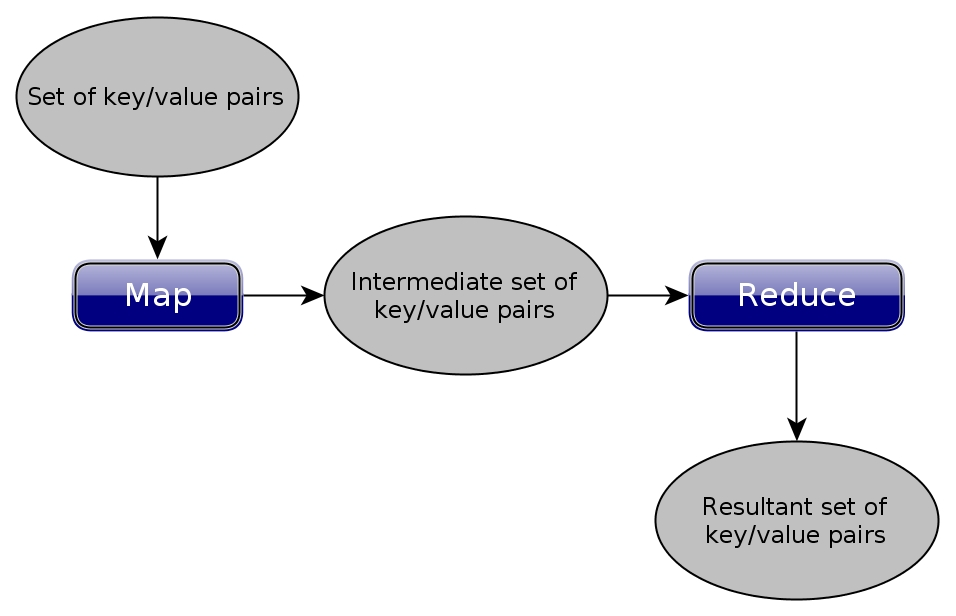
\includegraphics[width=\columnwidth]{img/mapReduce.jpg}
	\caption{Map and Reduce process.}\label{fig:mapReduce}
\end{figure}

\section{Hadoop}
Map and reduce functions are present in Lisp and others functional languages. Recently
the MapReduce paradigm have been implemented by several frameworks such as Greenplum
MapReduce~\cite{Greenplum:2008}, Aster Data~\cite{Aster:2011}, Nokia
Disco~\cite{Mundkur:2011}, Microsoft Dryad~\cite{Isard:2007}, and the one
open-source implemantation from Apache: Hadoop~\cite{hadoop}.

The Hadoop is a framework for reliable, scalable and distributed computing. It provide
an interface to implement the map and reduce functions in high-level which are internally
called as map and reduce tasks. It was designed for users focus on the implementation
those functions, without worrying about the issues involving the distributed computing.
All aspects involving the distributed computing and storage are left to the framework
such as split files, replication, fault tolerance and distribuition of the tasks.

There are two main components on Hadoop:
\begin{itemize}
	\item Hadoop Distributed File System(HDFS);
	\item Engine of MapReduce.
\end{itemize}

The HDFS stores all files in blocks, the block size is configurable per file, all
blocks of one file have the same block size except the last block. It is divided
in two components the \textit{NameNode} and \textit{DataNode}. The NameNode is placed
in one master machine, it stores all metedata and manages all DataNodes. The DataNode
stores data, when one DataNode starts it connects to theNameNode, then responds
to requests from the NameNode for filesystem operations.

The engine of MapReduce is responsible for parallel processing. It is constituted
by one master machine and slave machines, also called workers. The master
designates which slaves will receive map and reduce tasks with its respective input
blocks. The worker that receives map task is called mapper and the slave that receives
reduce task is called reducer.

\subsection{Job processing}

A job is a program in a high-level language(java, ruby or python) that implements
so the map and reduce functions. Initially the master machine receives jobs with
the relative input directory in the HDFS where are all files to be processed (inserted
previously in the HDFS). Then the master requests to the NameNode infomation
about the blocks and file locations, after that it deploys copies of the job across
several workers.

With the blocks information the map task is scheduled to a set of workers
with its respective input blocks. So the mappers process each input blocks, 
generate key/value intermediate pairs and append its in intermediate files. When
the mapper instance terminate it notifies the master. The master split the intermediate
files in blocks and shuffled them to the reducers to process. When all reducers
intances terminate processing, they append their result to the final output file.
The data flow between mappers and reducers are shown in Figure~\ref{fig:mrexecute}.

%%Fazer uma nova figura demonstrando o que foi escrito acima
\begin{figure}[htbp]
	\centering
	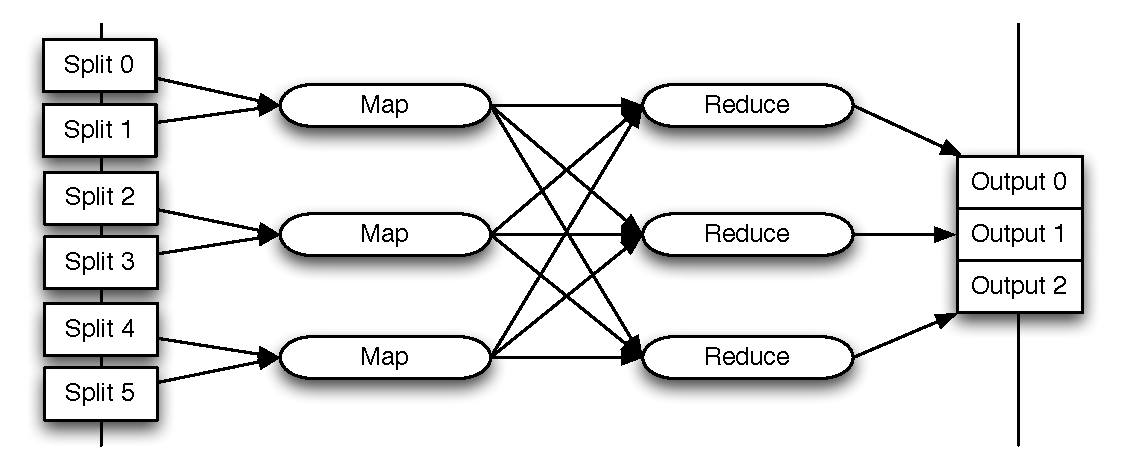
\includegraphics[width=\columnwidth]{img/mapreduce-en.pdf}
%    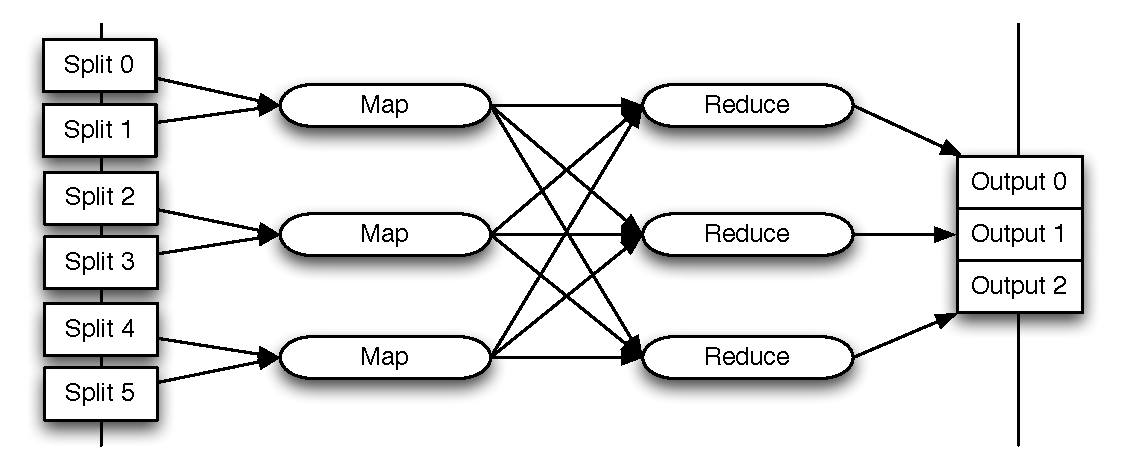
\includegraphics[bb=0 0 1280 960]{img/mapreduce-en.pdf}
	\caption{Execution of Map and Reduce operations}\label{fig:mrexecute}
\end{figure}

\subsection{MapReduce programing}

The whole processing is based on \tuple{key,value} pairs. The mappers receive the
file blocks, the mappers call the map function and pass the line number as key and
the line as the value, so the pair "line number/line content" is the \tuple{k1,v1}.
The map generate the intermediate result set of key and values \tuple{set(k2,v2)}, 
when the mappers finished all values for \textit{k2} are agrouped in a list and
the respective pair \tuple{k2, list(v2)} is generated. This pairs are sorted and
pass as input for reducers that generate the result set:

\begin{center}
\begin{tabular}{c c c c}
	\hline
	   map & $k1,v1$ & $\rightarrow$  & $set(k2, v2)$ \\
	   reduce & $k2, list(v2)$ & $\rightarrow$ & $set(v2)$ \\
	\hline
\end{tabular}
\end{center}

Eventually, when the map result are already available in memory, a local reduce
function \emph{Combiner} is used for optimization reasons, then all values for
determinated key are combined, resulting in a local set \tuple{k2, list(v2)}.
This function runs after the Map and before the Reduce functions on
every node that run map functions. The Combiner may be seen as a \emph{mini-reduce}
function, which operates only on data generated by one machine.

A good example of a MapReduce job is the Grep application listing~\ref{listing:mapper},
which receives as an input several textual documents and as an output a set of pairs
\tuple{Key,Value}, where each key is a different pattern found and the value is the
number of occurrences of the pattern in the files. The responsibility of the Mapper
is to find pattern in the files and the reduce is to sum the amount found each patterns.

The \code{map()} method has four parameters: \code{key}, which is never used; \code{value},
one line that contains the text to be processed; the \code{output}, which will receive
the output pairs and \code{reporter} for debug. The body of the method uses the class
\code{Pattern} to describe a desired pattern, the class \code{Matcher} to find this
pattern, when pattern are found the pair \tuple{matching, 1} is emited to
output.

\singlespacing
\begin{listing}[H]
\begin{minted}[frame=lines,framesep=2mm,fontfamily=courier,fontsize=\scriptsize]{java}
public class RegexMapper<K> extends MapReduceBase
			implements Mapper<K, Text, Text, LongWritable> {

    private Pattern pattern;
    private int group;

    public void configure(JobConf job)
    {
        pattern = Pattern.compile(job.get("mapred.mapper.regex"));
    }

    public void map(K key, Text value, OutputCollector<Text, LongWritable> output,
					Reporter reporter) throws IOException {
        String text = value.toString();
        Matcher matcher = pattern.matcher(text);
        while (matcher.find())
        {
            output.collect(new Text(matcher.group()), new LongWritable(1));
        }
    }
}
\end{minted}
\caption{Class RegexMapper packed in Hadoop~\cite{hadoop}} 
\label{listing:mapper}
\end{listing}

\doublespacing
The implementation of the reduce function is presented in Listing~\ref{listing:reducer}.
The \code{reduce()} method has also four parameters: \code{key}, which contains
a single matching string; \code{values}, a set containing all values associated
to the key (i.e. the matching); \code{output pair}, the resultant pair \tuple{matching,
total} and \code{reporter} for debug. The behavior of the method is straightforward,
it sums all values associated to the key and then writes a pair containing the same
key and the total of matching found.
\singlespacing
\begin{listing}[H]
\begin{minted}[frame=lines,framesep=2mm,fontfamily=courier,fontsize=\scriptsize]{java}
public class LongSumReducer<K> extends MapReduceBase
			 implements Reducer<K, LongWritable, K, LongWritable> {

    public void reduce(K key, Iterator<LongWritable> values,
                     OutputCollector<K, LongWritable> output, Reporter reporter)
                throws IOException {

    // sum all values for this key
    long sum = 0;
    while (values.hasNext())
    {
        sum += values.next().get();
    }

    // output sum
    output.collect(key, new LongWritable(sum));
  }

}
\end{minted}
\caption{Class LongSumReducer packed in Hadoop~\cite{hadoop}} 
\label{listing:reducer}
\end{listing}

\doublespacing
An example of the inputs and the outputs of both functions when applied to a
simple sentence is presented in Table~\ref{table:regexp}. We applied the following
regular expression: \\ \code{"[a-z]$*$o[a-z]$*$"}, this expression find the words that
contains the vowel \code{o} in the midle of them.

\begin{table}[H]
	\begin{center}
	\begin{tabular}{c p{.4\columnwidth} c p{.3\columnwidth} }
		\hline
		map & "Test for hadoop regular expression inside hadoop" & $\rightarrow$ & \tuple{for,1},\tuple{hadoop,1}, \tuple{expression,1}, \tuple{hadoop,1} \\
		reduce & \tuple{for,\{1\}}, \tuple{hadoop,\{1,1\}}, \tuple{expression,\{1\}} & $\rightarrow$ & \tuple{for,1},\tuple{hadoop,2}, \tuple{expression,1}\\
		\hline
	\end{tabular}
	\end{center}
	\caption{Regular expression example}
	\label{table:regexp}
\end{table}

% chapter chapter_name (end)
